\documentclass[11pt,a4paper]{report} 
\usepackage[ngerman]{babel} % deutsch und deutsche Rechtschreibung
\usepackage[utf8]{inputenc} % Unicode Text 
\usepackage[T1]{fontenc} % Umlaute und deutsches Trennen
\usepackage{textcomp} % Sonderzeichen wie Euro, Copyright, etc.
\usepackage[hyphens]{url} % Hyperlinks, eMail-Adressen, Pfadangaben
\usepackage{amssymb} % mathmatische Symbole
\usepackage{microtype} % reguliert Abstände zwischen Buchenstaben
\usepackage{graphicx} % wir wollen Bilder einfügen
\usepackage{float} % Umgebung die sich automatisch im Dokument an passenden Positionen bewegen (floaten)
\usepackage{emptypage} % Wirklich leer bei leeren Seiten

\usepackage{listings} % schöne Quellcode-Listings
% ein paar Einstellungen für akzeptable Listings
\lstset{basicstyle=\ttfamily, columns=[l]flexible, mathescape=true, showstringspaces=false, numbers=left, numberstyle=\tiny}
\lstset{language=C++} % Set your language (you can change the language for each code-block optionally)
% more information about listings: https://en.wikibooks.org/wiki/LaTeX/Source_Code_Listings

% Spezialpakete
\usepackage{epigraph} % Zum Positionieren von Bemerkungen links, rechts, oben und unten vom Text
\setlength{\epigraphrule}{0pt} % kein Trennstrich

% Seitenlayout
\usepackage[paper=a4paper,width=14cm,left=35mm,height=22cm]{geometry}
\usepackage{setspace}
\linespread{1.15}
\setlength{\parskip}{0.5em}
\setlength{\parindent}{0em} % im Deutschen Einrückung nicht üblich, leider

\newcommand{\phv}{\fontfamily{phv}\fontseries{m}\fontsize{9}{11}\selectfont}
\usepackage{fancyhdr} % ermöglicht schickere Header und Footer
\pagestyle{fancy}
\renewcommand{\chaptermark}[1]{\markboth{#1}{}}
\fancyhead[L]{\phv \leftmark}
\fancyhead[RE,LO]{\phv \nouppercase{\leftmark}}
\fancyhead[LE,RO]{\phv \thepage}
% Unten besser auf alles Verzichten
%\fancyfoot[L]{\textsf{\small \kurztitel}}
\fancyfoot[C]{\ } % keine Seitenzahl unten
%\fancyfoot[R]{\textsf{\small Medieninformatik}}

% Quellen aufteilen z.B. in Online-Quellen und Literaturverzeichnis
\usepackage{bibtopic} 

% Config 1: Times New Roman, gewohnter Font, ok tt und serifenlos
%\usepackage{mathptmx} 
%\usepackage[scaled=.95]{helvet}
%\usepackage{courier}

% Config 2: Palatino mit guten Fonts für tt und serifenlos
\usepackage{mathpazo} % Palatino, mal was anderes
\usepackage[scaled=.95]{helvet}
\usepackage{palatino }

% Config 3: New Century Schoolbook sieht auch nett aus (macht auch tt und serifenlos)
%\usepackage{newcent}

% Mehr Informationen zu Fonts: https://de.sharelatex.com/learn/Font_typefaces


% Zum Zeigen von Fehlern
\usepackage{soulutf8}
\newcommand*\falsch{\st}

% damit wir nicht so viel tippen müssen, nur für Demo 
\usepackage{blindtext} 

% Float-Objekte sollen die Section nicht verlassen in der sie eingefügt worden sind
\usepackage[section]{placeins}

\begin{document}

\begin{titlepage}
  \begin{center}
    % Kopf der Seite
    \parbox[t]{8cm}{
      % \textsf würde das Aussehen der ersten Seite ruinieren, 
      % wer will, soll das selbst außen rum machen...
      TH Nürnberg Georg Simon Ohm\\
      Fakultät Informatik \\
	}
    \vfill    
    {\LARGE Projektbericht} \\[0.5cm]
    {\large im Rahmen des Moduls IT-Projekt} \\[5mm]
    \rule{\textwidth}{1pt}\\[0.5cm]
    {\begin{spacing}{1.15} \huge \bfseries OHMComm \\Plattformunabhängiges Framework zur Audioübertragung \\ \end{spacing}}
    \rule{\textwidth}{1pt}    
    \vfill    
    \begin{tabular}{ll} % Mitte der Seite
      Vorgelegt von & Daniel, Jonas, Kamal \\
      am & bald \\
      Betreuer & Prof. Dr. M. Tessmann \\
    \end{tabular}    
    \vfill
\end{center}
\end{titlepage}
\cleardoublepage

% Zusammenfassung
\begin{abstract} 
Hier können wir eine kurze Zusammenfassung verfassen. Der restliche Text ist ein Blindtext. \blindtext
\end{abstract}

\tableofcontents


\chapter{Einführung} \label{chap:einf}
\epigraphhead[70]{\epigraph{Documentation is like sex: 
when it is good, it is very, very good; and when it is bad, 
it is better than nothing.}{\textit{Dick Brandon}}}

Latex ist verglichen mit anderen Textverarbeitungsprogrammen nicht gerade intuitiv bedienbar. Die Lernkurve ist zwar steil, jedoch lohnt sich der Aufwand. Man bekommt qualitativ hochwertige Dokumente in Buchdruckqualität.
\
\section{Referenzen in Latex} \label{sec:ref}
Referenzieren in Latex sollte geübt sein. Referenzieren bedeutet Verweisen. Häufig verweist man in seinen Text auf andere Kapitel, Bilder, Tabellen oder Listenings. Man sollte niemals mit einer hart kodierten Zahl auf etwas verweisen. Die Referenz wird ungültig, falls sich die Reihenfolge ändert. Latex bietet Möglichkeiten zum Referenzieren mit dem Befehl \verb|ref| und \verb|label|. Beispiel: Wir befinden uns gerade im Kapitel \ref{chap:einf} und in der Section \ref{sec:ref}. Für das korrekte Referenzieren muss i.d.R. zweimal hintereinander kompiliert werden! Beim ersten Kompilieren erscheinen statt der Referenz nur \verb|??|. Man kann auf die Seitenzahl verweisen. So kann zum Beispiel auf Seite \pageref{fig:templateprozess} in Abbildung \ref{fig:templateprozess} ein hässliches Bild sehen.


\section{Aufzählungen} \label{sec:num}
\begin{itemize}
	\item Aufzählungen sehen in Latex sehr schick aus.
	\item Aufzählungen sehen in Latex sehr schick aus.
	\item Aufzählungen sehen in Latex sehr schick aus.
\end{itemize}

\section{Durchgestrichener Text} \label{sec:durchgestrichen}
\falsch{Durchgestrichener Text könnte auch mal nützlich sein.}

\chapter{Der Hauptteil} \label{chap:hauptteil}
\epigraphhead[70]{\epigraph{Surely, somewhere, somehow, in the history of 
computing, at least one manual has been written that you could at least 
remotely attempt to consider possibly glancing at.}{\textit{Adam Rixey}}}

Wir beginnen wieder ein neues Kapitel. Die Kapitelanordnung ist rein zufällig und dient nur zu Demonstrationszwecken.
Es folgt ein Blindtext: \blindtext

\section{Zitieren} \label{sec:zit}
Zitate müssen deutlich gekennzeichnet werden ~\cite[S. 12ff.]{gockel}. Zum Zitieren wird in diesem Dokument die Haward-Zitierweise~\cite[S. 12ff.]{wikiciting} verwendet. Hierbei wird der Nachname des Autors, Erscheinungsdatum und die Seite angegeben ~\cite[S. 12ff.]{wikipedia}.

\section{Abkürzungen} \label{sec:abk} Abkürzungen werden bei erster Verwendung vollständig ausgeschrieben wie z.B. \textit{Christliche Soziale Union} (CSU). Danach kann man auf die Abkürzung, in diesem Fall CSU, zugreifen. Grundsätzlich sollten Abkürzungen sparsam verwendet werden.
\newpage

\section{Tabellen} \label{sec:tab}
Tabellen sehen auch schick aus.
\begin{table}[htbp] % htbp ~ here, top, bottom, page (Bei dieser Angabe handelt es sich um eine Prioritätenangabe bezüglich der Positionierung. Latex soll versuchen die Tabelle "here" zu positionieren. Wenn das nicht klappt dann "top", dann "buttom" und dann "page".)
\centering
\begin{tabular}{|p{4.5cm}|c|r|} % Anzahl der Spalten: Spalte 1 hat Breite von 4.5, Spalte 2 ist so breit wie nötig und centered, Spalte 3 ist so breit wie nötig und right-aligned
\hline
\multicolumn{1}{|c|}{\textbf{Plattform}} & 
\multicolumn{1}{|c|}{\textbf{\LaTeX-Distribution}} & 
\multicolumn{1}{|c|}{\textbf{Editor}} \\ \hline \hline % Größerer Abstand zwischen Head und Inhalt
Linux/Unix & TeX Live & Texmaker \\\hline
MacOSX     & \multicolumn{2}{|c|}{Super Toll} \\\hline
Windows    & MiKTeX   & Any other cool Tool \\\hline   
\end{tabular}
\caption{\LaTeX-Distributionen und Editor je Plattform}
\label{tab:example1}
\end{table}
Tabellen sind natürlich auch referenzierbar siehe Tabelle \ref{tab:example1}.

\section{Hervorhebungen} \label{sec:hervorheben}
Einzelne Wörter können mit dem \verb|verb|-Befehl hervorgehoben werden.

\section{Bilder}  \label{sec:bil}
Bilden werden, wie die meisten Objekte in Latex, in Float-Umgebungen eingesetzt. Das heißt Latex bestimmt selbst, wo sich das Bild im Dokument positioniert. Wie fast alle Objekte lassen sich auch in Bilder referenzieren. Zum Beispiel sieht man auf Abbildung \ref{fig:templateprozess}, dass nicht alle Menschen gut zeichnen können.

\begin{figure}[htp] % here, top, page - https://en.wikibooks.org/wiki/LaTeX/Floats,_Figures_and_Captions
\centering
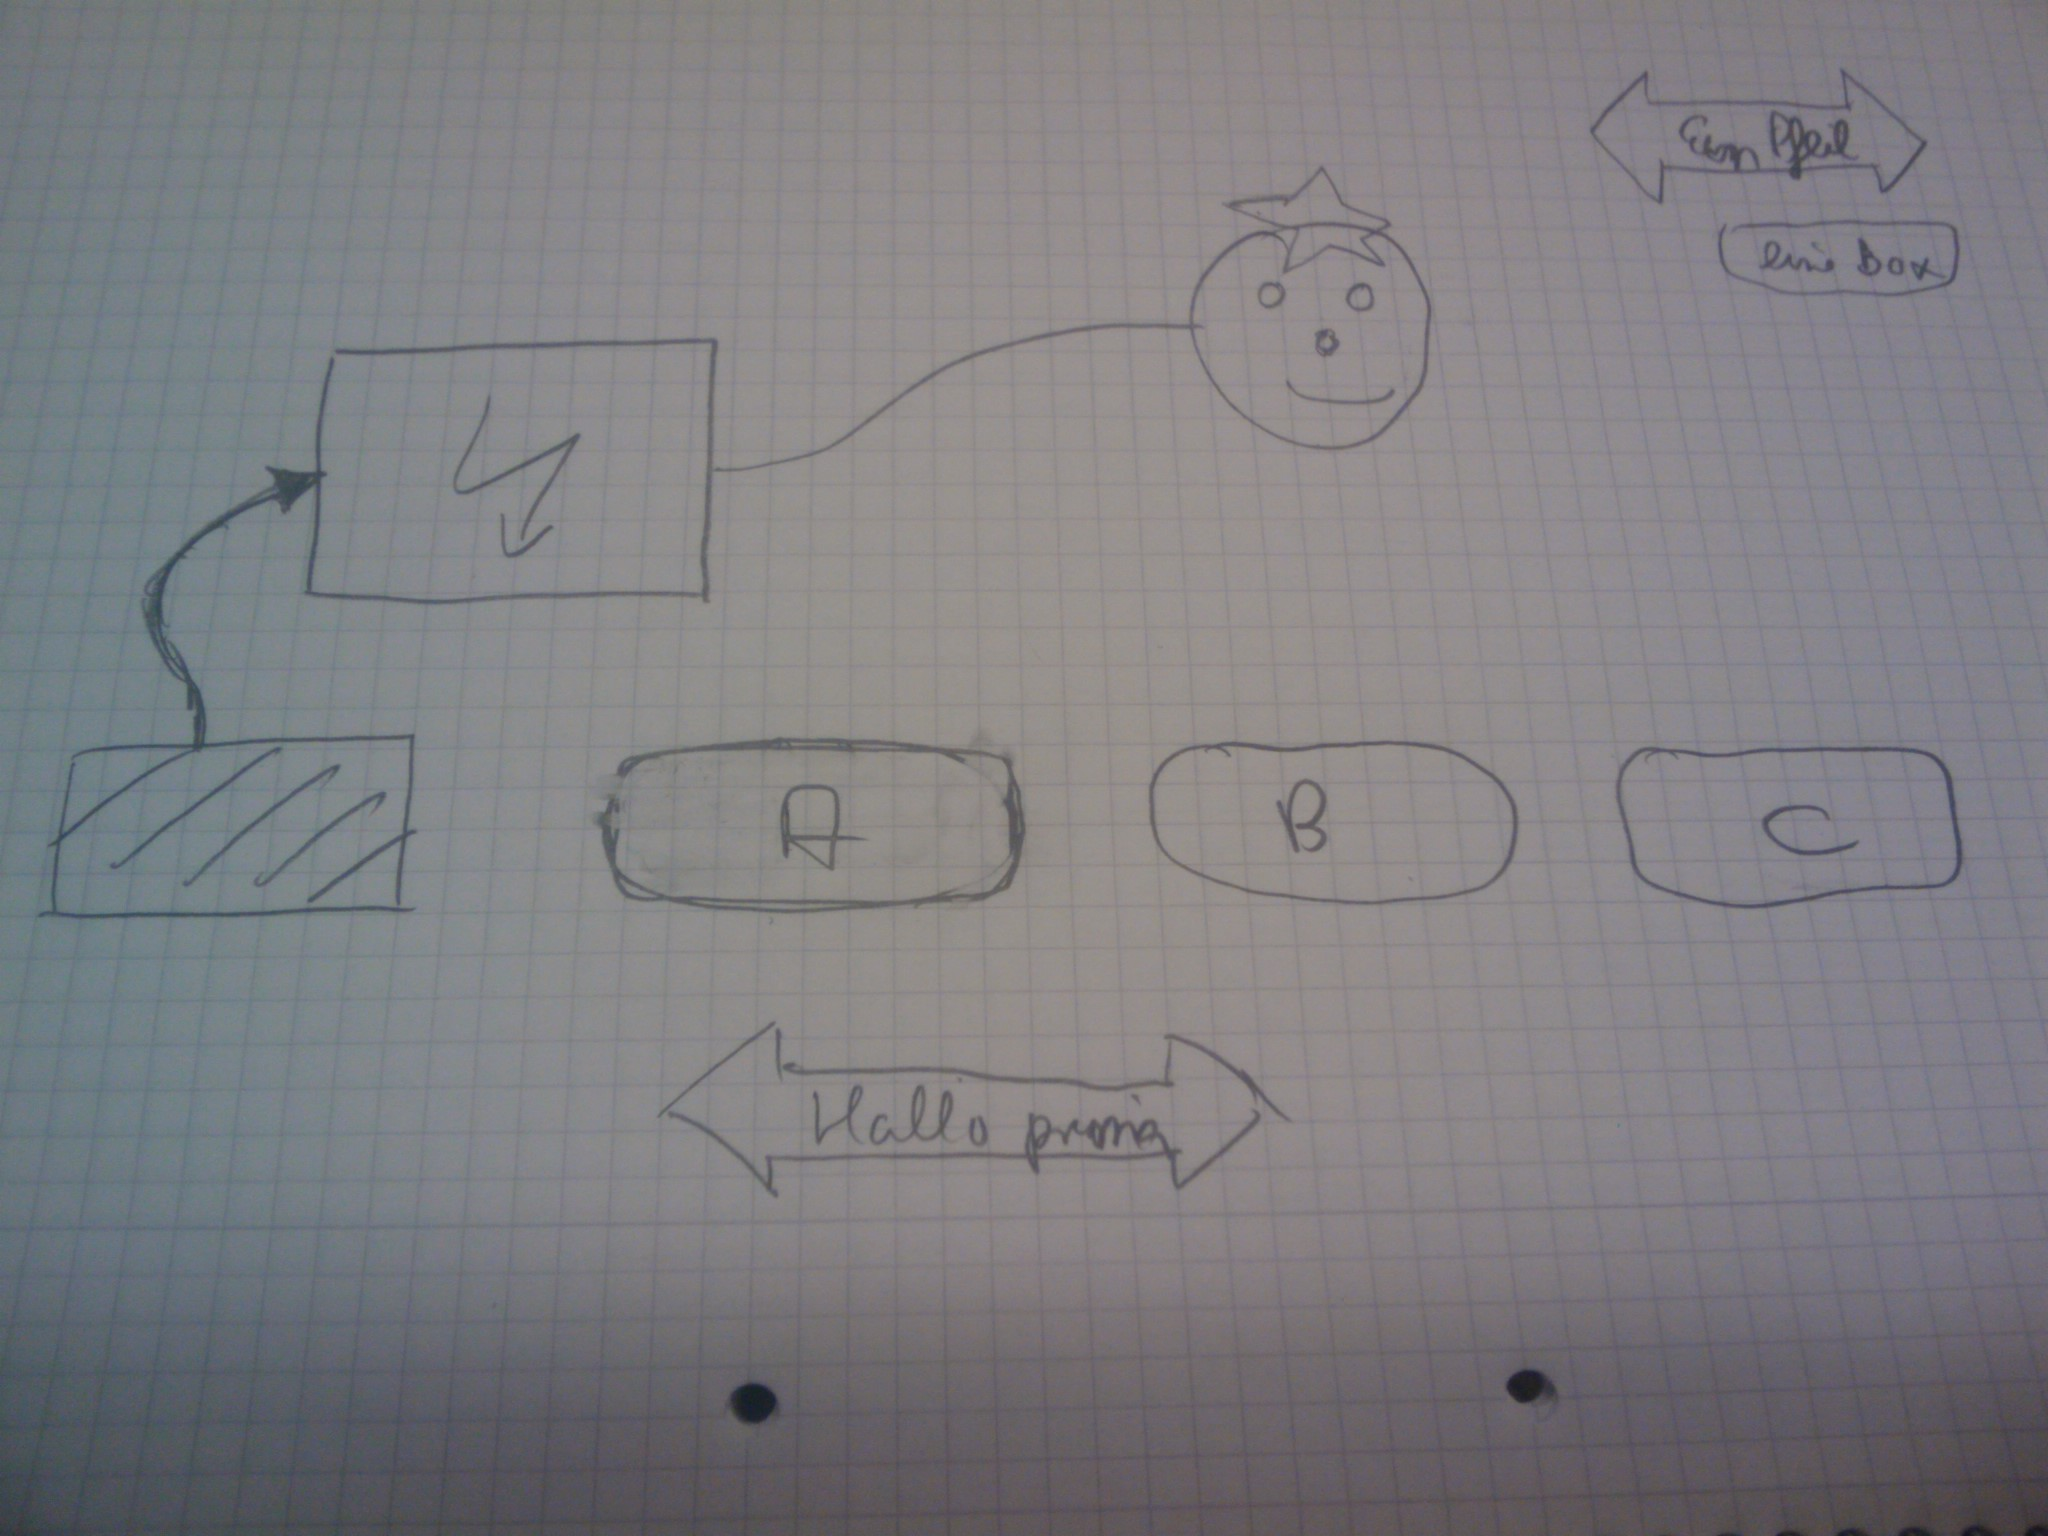
\includegraphics[width=.9\textwidth]{images/zeichnungdraft} % Grafikgröße entspricht 0.9 Textbreite, dateiname ist templateprozess
\caption{Dateien zur Erstellung des Templates}
\label{fig:templateprozess}
\end{figure}

\subsection{Seitenlayout}
Das Seitenlayout ist definiert als A4-Paper mit 14 cm Textbreite, Texthöhe von 22 cm und linksseitigen Abstand von 3.5 cm. Außerdem wird mit \verb|linespread{1.15}| der Zeilenabstand auf ca. 1.5 gesetzt.

\subsection{Bindestriche}
Einfache Bindestriche werden zur Worttrennung eingesetzt. Zum Beispiel Flug-simulator. Der Gedankenstrich wird bei Einschüben eingesetzt und ist --- wie man sieht --- länger als der normale Bindestrich.

\subsection{Listings}
Lange Listings sind nie schön wie z.B. Listing \ref{code:ggtaua}.
\begin{lstlisting}[caption={Listenings sind toll}\label{code:ggtaua},captionpos=b]
#include <stdio.h>
#define N 10
    using namespace std;
    // This creates a Fibonacii series
    void Fibonacii::create_series(void){
    data.push_back(0);
    data.push_back(1);
    for (int i = 2; i < size; ++i)
    {
    /* code */
    data.push_back(data[i - 2] + data[i - 1]);
    }
    }
    // This is a constructor
    Fibonacii::Fibonacii(int s){
    size = s;
    }
    // This method is used to print the series
    void Fibonacii::get_data(void){
    for (long i: data)
    cout << i << endl;
    }
\end{lstlisting}


\bibliographystyle{apalike} % Literaturverzeichnis
\begin{btSect}{thesis} % mit bibtopic Quellen trennen
\section*{Literaturverzeichnis}
\btPrintCited
\end{btSect}
\begin{btSect}{online}
\section*{Online-Quellen}
\btPrintCited
\end{btSect}

\end{document}